% This LaTex template is designed to standardize student report submission for CaYPT individual selection. It is based on the physical review package LaTex template (revtex).
% Edited by Jim Chen
% Rev A, Mar, 2024

\documentclass[prl,twocolumn,amsmath,amssymb,superscriptaddress]{revtex4-2}

% You may use additional packages as you see fit
\usepackage{graphicx}
\usepackage{verbatim}
\usepackage{braket}
\usepackage{epsfig}
\usepackage{epstopdf}
\usepackage{amsfonts}
\usepackage{amsthm}
\usepackage{amsmath}
\usepackage{amssymb}
\usepackage{color}
\usepackage[usenames,dvipsnames,svgnames,table]{xcolor}
\usepackage{hyperref}
\hypersetup{colorlinks=true,linkcolor=NavyBlue,citecolor=BrickRed,urlcolor=NavyBlue}
\usepackage{dsfont}
\usepackage{color}
\usepackage{grffile}
\usepackage{bm}
\usepackage{lipsum}
%end of packages

% Start of the main text. Replace /lipsum[] with your text. The main text should be kept at less than 6 pages.
\begin{document}

\title{PHY180: Pendulum Project}
\date{\today}

\begin{abstract}
By attaching a magnet to a string, and allowing it to move over magnets on a base, interesting motion patterns emerge. In this report, we first model the magnetics and mechanics in the system, before investigating motion in both single and double magnet cases.
\end{abstract}

\maketitle

\section{Introduction}
The problem statement for \textit{Magnetic Assist} reads:

\begin{center}
{\it ``Attach one or two magnets to a non-magnetic and non-conductive base such that they attract a magnet suspended from a string. Investigate how the motion of the moving magnet depends on relevant parameters."}
\end{center}

As you might expect, when you attach magnets in such an orientation, the equilibrium point of the pendulum shifts---thus the name \textit{Magnetic Assist}.

If we're too look at the system from a forces perspective, the reason for this becomes more obvious.

\begin{figure}[htb]
    \includegraphics[width=0.8\linewidth]{force_diagram.png}
    \label{fig:Force diagram}
\end{figure}

Now, the interesting and unexpected parts of this system emerge in motion, not in the bland qualitative, so we will move on to modelling the system.

\section{Mechanics}
Having now solved for the magnetic interaction, we can proceed to analyze the mechanics of the pendulum. To do this, we first solve for the Euler-Lagrange equations of motion for the pendulum.

\begin{equation}
\begin{split}
    \frac{d}{dt}\left(\frac{\partial L}{\partial \dot{\theta}}\right) &= \frac{\partial L}{\partial \theta} \\
    \frac{d}{dt}\left(\frac{\partial L}{\partial \dot{\phi}}\right) &= \frac{\partial L}{\partial \phi}
\end{split}
\end{equation}

\begin{equation}
    \begin{split}
        \ddot{\theta} &= sin(\theta)cos(\theta)\dot{\phi}^2 - \frac{g}{l}sin(\theta)\\
        \ddot{\phi} &= \frac{-2\dot{\theta}\dot{\phi}cos(\theta)}{sin(\theta)}
    \end{split}
    \label{equation:motion}
\end{equation}

Next, we project the cartesian magnetic force onto the tangent plane of the pendulum's spherical projection:

\begin{equation}
\begin{split}
    F_\theta &= F_x \cos\theta \cos\phi + F_y \cos\theta \sin\phi + F_z \sin\theta \\
    F_\phi &= -F_x \sin\phi + F_y \cos\phi
\end{split}
\end{equation}

Lastly, we define relevant damping terms in the system, including Coulomb friction, air resistance, viscous damping, and electromagnetic damping (eddy current damping).

\begin{equation}
    \begin{split}
        \ddot{\theta}_d &= \mu_c sgn(\dot{\theta}) + \mu_a \dot{\theta} + \mu_v \dot{\theta}^2 + \mu_e \dot{\vec{B}}^2 \\
        \ddot{\phi}_d &=\mu_c sgn(\dot{\phi}) + \mu_a \dot{\phi} + \mu_v \dot{\phi}^2 + \mu_e \dot{\vec{B}}^2
    \end{split}
    \label{equation:damping}
\end{equation}

Given this complete equation of motion, we can solve the ordinary differential equations numerically using the Runge-Kutta-Fehlberg adaptive method.

We implement our code in Python, but compile it using Numba similarly to the field and Lorentz integrations. Compiled performance integrates a 8 second simulation in typically under a second timescale.

\section{Experiment}
Our experimental setup consists of a camera mounted on a tripod over which the pendulum is suspended using high-tension wires. A picture can be seen in Figure \ref{fig:experiment_setup}.

\begin{figure}[htb]
    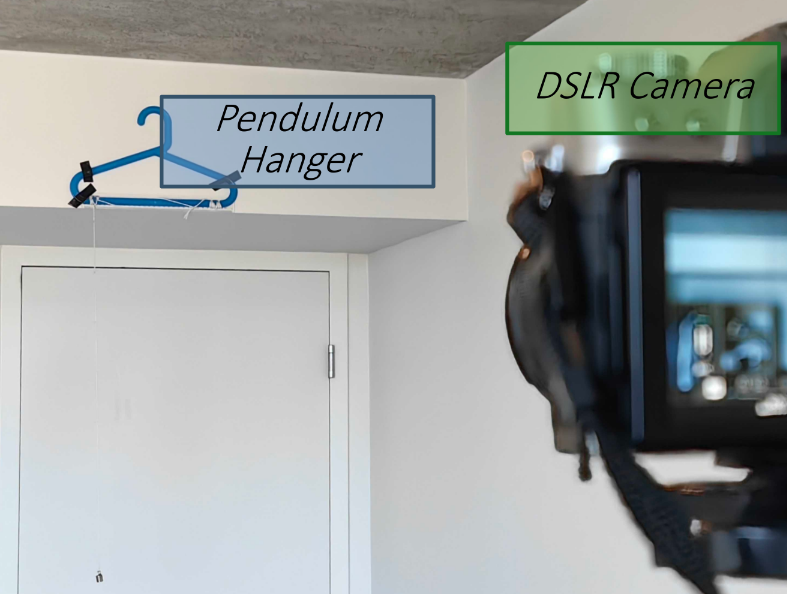
\includegraphics[width=0.66\linewidth]{setup.png}
    \caption{Picture of experimental setup.}
    \label{fig:experiment_setup}
\end{figure}

We use OpenCV to apply a computer vision algorithm to the video feed to obtain the pendulum's position in real-time.

Since we've removed shadows using our observer light-source, as well as increased contrast through the paper plane on top of the base magnets, the edge detection algorithm works very well. While we found challenges removing the suspension wire in the captured video, we were able to use a high aperture lens (35mm/1.4) to effectively pull it out of focus.

\begin{figure}[htb]
    \includegraphics[width=0.9\linewidth]{tracking.png}
    \caption{L: Frame of camera capture and found position R: image of edge-detection frame.}
    \label{fig:tracking}
\end{figure}

Having found the position on the projected image, we can use the pixel coordinates to calculate the pendulum's position in the real world.


\begin{figure}[htb]
    \includegraphics[width=0.6\linewidth]{trig_transform.png}
    \caption{Geometry of setup.}
    \label{fig:coordtrans}
    \vspace{-30pt}
\end{figure}


\begin{equation}
    \phi = \tan^{-1} \left(\frac{p_x}{p_y} \right) \\
\end{equation}
\begin{equation}
    \angle l_p = \tan^{-1} \left(\frac{s_h \| p \|}{f p_w} \right)
\end{equation}
\begin{equation}
    \theta = \angle l_p + \arcsin \left(\frac{l_c}{l_p} \sin \angle l_p \right)
\end{equation}
To verify this, we manually measure angles and compare to the calculated values. Results can be seen in Fig. \ref{fig:verify_coords}.

\begin{figure}[htb]
    \includegraphics[width=0.75\linewidth]{verify_track.png}
    \caption{Verification of calculated angles.}
    \label{fig:verify_coords}
\end{figure}

\newpage
\subsection{Characterization}
We characterize the relevant constants in the system.

Firstly, damping constants were fit obtaining damping curves experimentally across multiple trials and fitting relevant constants.

\begin{figure}[htb]
    \includegraphics[width=1\linewidth]{RMSE_fitting.png}
    \caption{Multiple damping characterization trials using minimized constants. RMSE 0.03. Eddy damping is also fit.}
    \label{fig:damping}
\end{figure}

Next, we fit the magnetic dipole moment, $\vec{m}$, to our magnets. We do this by using a 3-axis teslameter ($\mu T$ accuracy) with baseline measurement. We find $m =0.0987 Am^2$, or alternatively $M=1.22 \times 10^6 A/m$.

\begin{figure}[htb]
    \includegraphics[width=\linewidth]{magnet_fit.png}
    \caption{Fit of magnetic dipole moment. N=3 in experiment.}
    \label{fig:fit_field}
\end{figure}

\section{Analysis}
As per the problem statement, we will be analyzing the pendulum's motion in both the  single and double attracting magnet configuration. Analysis of the single-magnet regime is largely in the frequency domain, while analysis of the double-magnet regime is focused on chaos.

\subsection{Single Magnet Regime}

\begin{figure}[htb]
    \includegraphics[width=\linewidth]{eddy_currents.png}
    \caption{Theory vs. experimental for a single-magnet case. Oscillations in experimental are due to off-angle camera.}
\end{figure}

The single magnet regime can be roughly described to be composed of 3 phases: a simple-pendulum phase, a inter-phase where the frequency of oscillation rises, and a trembling phase where the frequency of oscillation plateaus.


This can be best visualized by plotting to peak of a fourier transform across time bins.

In Fig. \ref{fig:phases}, we've labeled each phase. These changes can be explained by changes in the amplitude of magnetic force as $\theta$ decreases, affecting the centripetal force acting on the pendulum. Eventually this force asymptotes due to the diminishing change $\theta$ has on the distance between the magnets, causing the trembling.

\begin{figure}[htb]
    \includegraphics[width=\linewidth]{single_phases.png}
    \caption{Visualization of the different phases in the pendulum motion.}
    \label{fig:phases}
\end{figure}

We can see that our simulation can successfully predicts the frequency characteristics of the system in Fig. \ref{fig:freq_magnet}. Unfortunately, we only have one experimental datapoint for magnet strength due to being unable to eliminate compounding factors such as mass and geometry when changing the magnet strength.

\begin{figure}[htb]
    \begin{minipage}{0.45\linewidth}
        \includegraphics[width=\linewidth]{frequency_time.png}
    \end{minipage}%
    \begin{minipage}{0.45\linewidth}
        \includegraphics[width=\linewidth]{magnet_strength.png}
    \end{minipage}
    \caption{L: Frequency over time. R: Tremble frequency with magnetic strength.}
    \label{fig:freq_magnet}
\end{figure}

\newpage
It should be noted that in this single magnet analysis we only investigated the least eccentric mode, as it is the most revealing. Our simulation does however accurately model the pendulum in situations of increased eccentricity as seen in Fig. \ref{fig:eccentricity}.

\begin{figure}[htb]
    \includegraphics[width=\linewidth]{increasing_eccentricity.png}
    \caption{Visualization of the different phases in the pendulum motion.}
    \label{fig:eccentricity}
\end{figure}
\subsection{Double Magnet Regime}

The double magnet regime of this system is more interesting. Due to the prevalence of transient chaos, comparing simulation transients with experimental transients not meaningful (they always diverge in chaotic regions).

To analyze this, we use \textit{Fractal basins}. In a fractal basin, each pixel represents a separate simulation where the initial conditions coincide with the pixel's X and Y coordinate. The color of that pixel represents the final osition of the pendulum along the x-axis.

\begin{figure}[htb]
    \centering
    \includegraphics[width=\linewidth]{fractal.png}
    \caption{Visualization of end states based on initial position.}
    \label{fig:fractal}
\end{figure}

In Fig. \ref{fig:fractal} you see a fractal basin formed by a set of conditions in the double-magnet regime.

\subsection{Basin Zones}
One of the interesting implications is that the path the pendulum takes stays consistent within basin zones. For instance, as seen in Fig. \ref{fig:basin_zone}, the pendulum loops around the right magnet before settling on the left (thus the green patch).

\begin{figure}[htb]
    \centering
    \includegraphics[width=\linewidth]{basin_zone.png}
    \caption{An example of a basin zone.}
    \label{fig:basin_zone}
    \vspace{-20pt}
\end{figure}

\subsection{Key Parameter Interactions}
First, we vary the length of the pendulum string. As the string length increases, the basin zone increases (as the initial potential energy decreases). The result can be seen in Fig. \ref{fig:length_interaction}.

\begin{figure}[htb]
    \begin{minipage}{0.45\linewidth}
        \includegraphics[width=\linewidth]{start_length.png}
    \end{minipage}%
    \hspace{5pt}
    $\rightarrow$
    \begin{minipage}{0.45\linewidth}
        \includegraphics[width=\linewidth]{end_length.png}
    \end{minipage}
    \caption{Change in basin as length is increased.}
    \label{fig:length_interaction}
\end{figure}

Next, varying the strength of our magnet, we see that the basin zone grows in Fig. \ref{fig:strength_interaction}.
\begin{figure}[htb]
    \begin{minipage}{0.45\linewidth}
        \includegraphics[width=\linewidth]{start_strength.png}
    \end{minipage}%
    \hspace{5pt}
    $\rightarrow$
    \begin{minipage}{0.45\linewidth}
        \includegraphics[width=\linewidth]{end_strength.png}
    \end{minipage}
    \caption{Change in basin as magnet strength is increased.}
    \label{fig:strength_interaction}
\end{figure}
\newpage
\subsection{Gravity as a Third Attractor}

Another interesting phenomenon occurs when you move the magnets apart from each other. As is visible in the basin shown in Fig. \ref{fig:3rd_attractor}, a third color emerges, turqoise, symbolizing an end state between the two magnets.

\begin{figure}[htb]
    \centering
    \vspace{-10pt}
    \includegraphics[width=0.8\linewidth]{3rdattractor.png}
    \caption{Fractal basin where a third attractor has emerged. Patterns at edges are due to lack of integration time.}
    \label{fig:3rd_attractor}
\end{figure}

This can be explained through potential hills.

We can use the magnetic dipole energy equation (as this is purely a qualitative investigation) and gravitational potential equation (Eq. \ref{eq:mag_poten}-\ref{eq:grav_pot}).

\begin{equation}
    U_B = \vec{B} \cdot \vec{m}
    \label{eq:mag_poten}
\end{equation}
\begin{equation}
    U_g = -mg \sqrt{l^2-x^2-y^2}
    \label{eq:grav_pot}
\end{equation}

Through this, we can solve for the potential energy as a function of the pendulum's position. A 3D plot of this can be seen in Fig. \ref{fig:3dhills}.
\vspace{-10pt}
\begin{figure}[htb]
    \centering
    \includegraphics[width=0.8\linewidth]{3dhills.png}
    \caption{A 3D plot of the calculated potential hills of a double-magnet system.}
    \label{fig:3dhills}
\end{figure}

\newpage
In Fig. \ref{fig:3rddip}, we observe that as we move the magnets away from each other, a third dip in the energy forms, creating a stable equillibrium position.

\begin{figure}[htb]
    \centering
    \includegraphics[width=0.7\linewidth]{3rddip.png}
    \caption{A cross section of the potential hill where a third attractor is visible.}
    \label{fig:3rddip}
\end{figure}

\section{Conclusion}
In this report, we investigated the motion of a suspended magnet under the influence of attractive magnets placed on a base.

We first developed a comprehensive model for magnetic interactions using a current cylinder model. For the mechanics, we derived the equations of motion using Euler-Lagrange formalism and incorporated various damping effects. For the experimental setup, we designed a novel single-camera computer vision approach, with which we collected relevant data.

After which we analyzed both the single and double magnet regimes in relation to numerous parameters.

If I were to be selected, future work during IYPT preparation would largely include collecting more experimental data.

Lastly, thank you to the people I received feedback for regarding this project, and the COC for organizing CaYPT.

\bibliography{refs.bib}{}
\bibliographystyle{plain}
\end{document}
